\documentclass[twocolumn]{article}
\usepackage[english]{babel}
\usepackage[utf8]{inputenc}
\usepackage{amsmath,amssymb,physics,mathtools,blindtext,graphicx,float}
\usepackage[a4paper,total={7.5in,10in}]{geometry}
\usepackage[labelfont=bf]{caption}

\begin{document}
\begin{large}
\begin{center}
    \includegraphics[scale=0.5]{Layer1.png}
\end{center}


No net flux through layer 1 gives 
\begin{equation}
    \begin{split}
        0 &= 2\epsilon_1\sigma T_1^4 + (1-\epsilon_1)\sigma T_0^4 - \epsilon_0\sigma T_0^4 \\ 
        &= 2\epsilon_1\sigma T_1^4 - \epsilon_0\epsilon_1\sigma T_0^4
    \end{split}
\end{equation}
and zero net flux through the top of the atmosphere gives 
\begin{equation}
    (1-\epsilon_1)\epsilon_0\sigma T_0^4 + \epsilon_1\sigma T_1^4 = S
\end{equation}
where $S$ is the average flux density of the incoming solar radiation, $S=239.05$ Wm$^{-2}$. These two equations are linear in $\sigma T_0^4$ and $\sigma T_1^4$ and can be easily solved to give
\begin{equation}
    ...
\end{equation}

This model can be generalized by adding more layers. For $N$ layers, the temperatures in the different layers $T_i$ will be given by the solution to the $N+1$ dimensional linear system of equations
\begin{equation}
    A\mathbf{x} = \mathbf{b}
\end{equation}
where $x_i = \sigma T^4$. The first row of $A$ corresponds to the equation of no net flux through the top of the atmosphere:
\begin{equation}
    \sum_{j=0}^{N}A_{0,j}x_j = S
\end{equation}
where $A_{0,j}x_j$ is the contribution of layer $j$ to this equation, i.e.
\begin{equation}
    A_{0,j}x_j = \epsilon_j(1-\epsilon_{j+1})(1-\epsilon_{j+2})\dots(1-\epsilon_{N})\sigma T_j^4.
\end{equation}
Row $i>0$ corresponds to the equation of no net flux through layer $i$. Its own contribution to this equation is
\begin{equation}
    A_{i,i}x_i = 2\epsilon_i\sigma T_i^4
\end{equation}
It is then convenient to look at the contribution of layers $j<i$ and layers $j>i$ seperately. For $j<i$, the contribution from layer $j$ to the flux through layer $i$ is 
\begin{equation}
    \begin{split}
        A_{i,j}x_j &= \epsilon_j(1-\epsilon_{j+1})(1-\epsilon_{j+2})\dots(1-\epsilon_{i})\sigma T_j^4 \\ 
        &\hspace{0.3cm} -\epsilon_j(1-\epsilon_{j+1})(1-\epsilon_{j+2})\dots(1-\epsilon_{i-1})\sigma T_j^4 \\ 
        &= -\epsilon_i\epsilon_j(1-\epsilon_{j+1})(1-\epsilon_{j+2})\dots(1-\epsilon_{i-1})\sigma T_j^4.
    \end{split}
\end{equation}
The flux going out of layer $i$ is positive and the flux going into it is negative. For $j>i$, we have similarily
\begin{equation}
    \begin{split}
        A_{i,j}x_j &= \epsilon_j(1-\epsilon_{j-1})(1-\epsilon_{j-2})\dots(1-\epsilon_{i})\sigma T_j^4 \\ 
        &\hspace{0.3cm} -\epsilon_j(1-\epsilon_{j-1})(1-\epsilon_{j-2})\dots(1-\epsilon_{i+1})\sigma T_j^4 \\ 
        &= -\epsilon_i\epsilon_j(1-\epsilon_{j-1})(1-\epsilon_{j-2})\dots(1-\epsilon_{i+1})\sigma T_j^4.
    \end{split}
\end{equation}
The equation for zero net flux through layer $i$ is then
\begin{equation}
    \sum_{j=0}^{N}A_{i,j}x_j = 0.
\end{equation}
The vector $\mathbf{b}$ is thus given by $\mathbf{b} = (S,0,0,\dots,0)$. Having set up the matrix $A$ and vector $\mathbf{b}$, we could solve for the temperatures in each layer. However, the emissivities can depend on various physical variables such as temperature, density and wavelength of the radiation. Here, it will be assumed that the emissivities $\epsilon_j$ only depend on the densities of the layers $\rho_j$ and their thickness $h_j$ by the following relationship:
\begin{equation}
    \epsilon_j = \alpha\rho_jh_j.
\end{equation}
where $\alpha$ is a constant such that $0\leq\epsilon_j\leq 1$. This however entails a complication because of the fact that the density of air depends on its temperature, which is the variable we are trying to solve for. How this is solved is explained later. 

The density of layer $j$ can be calculated from the ideal gas law and Boltzmann statistics:
\begin{equation}
    \begin{split}
        &P_j = \rho_jk_BT_j/m \\ 
        &P_j = P_{j-1}e^{-mgh_{j-1}/k_BT_{j-1}}.
    \end{split}
\end{equation}
Here $P_j$ is the pressure in layer $j$, $k_B$ is the Boltzmann constant and $m$ is the average mass of an air molecule, $m=4.8\cdot 10^{-26}$ kg. If we know $P_0$ and the temperature in each layer, we can calculate the density in each layer recursively with:
\begin{equation}
    \rho_j = \frac{mP_{j-1}}{k_BT_j}e^{-mgh_{j-1}/k_BT_{j-1}}.
\end{equation}
The pressure and density at the surface are assumed to be $P_0=101.3$ kPa and $\rho_0=1.225$ kg/m$^3$, respectively.

%The parameters of this model are the number of layers, $N$, and the emissivity of each layer $\epsilon_i$. The emissivities can depend on various physical variables such as temperature, density and wavelength of the radiation. If it is temperature dependent, the system of equations becomes non-linear.

\subsection*{Results}
\begin{figure}[!b]
    \begin{center}
        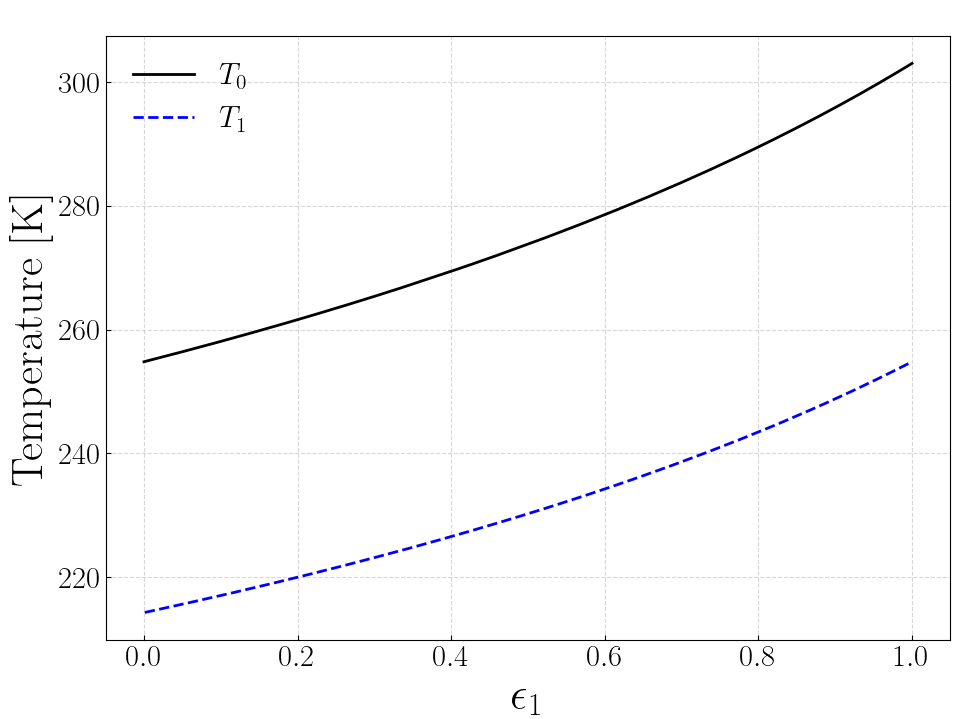
\includegraphics[scale=0.35]{OneLayer.png}
    \end{center}
    \caption{The surface temperature $T_0$ and the temperature in the layer $T_1$, as a function of the emissivity of that layer $\epsilon_1$.}
    \label{9maj1827}
\end{figure}
The method was tested for one layer and different emissivities, $\epsilon_1$, of that layer. The surface of the earth had emissivity $\epsilon_0=1$. The result can be seen in figure \ref{9maj1827}. The span of the surface temperature for different emissivities is $255-303$ K which at least contains the estimate for the surface temperature from measured data, $287.2$ K. The temperature in the layer, $T_1$, is roughly $40-50$ K lower than $T_0$. This seemed to be a general characteristic of this model, i.e. that the higher layers always had lower temperature than the layers below. 



























%\begin{equation*}
%    \begin{split}
%        &T_i^\text{Vi,In} = T_{i+1}^\text{Vi,In}e^{-\sigma_\text{Vi}\rho_ih} \\ 
%        &T_i^\text{IR,In} = \left(T_{i+1}^\text{In,IR}+\frac{E_{i+1}}{2}\right)e^{-\sigma_\text{IR}\rho_ih} \\ 
%        &T_i^\text{Out} = \left(T_{i-1}^\text{Out}+\frac{E_{i-1}}{2}\right)e^{-\sigma_\text{IR}\rho_ih} \\ 
%        &E_i = \left(\frac{E_{i-1}+E_{i+1}}{2}+T^\text{Out}_{i-1}+T^\text{IR,In}\right)\left(1-e^{-\sigma_\text{IR}\rho_ih}\right) \\ 
%        &\hspace{5.2cm} + T_{i+1}^\text{Vi,In}\left(1-e^{-\sigma_\text{Vi}\rho_ih}\right)
%    \end{split}
%\end{equation*}
%Given an initial condition $T_N^\text{Vi,In}$, we can easily calculate all other $T_i^\text{Vi,In}$ if we know $\rho_i$. The other three equations can be written as 
%\begin{equation}
%    \begin{split}
%        &T_i^\text{IR,In} - g_iT_{i+1}^\text{IR,In}-\frac{g_i}{2}E_{i+1} = 0 \\ 
%        &T_i^\text{Out} - g_iT_{i-1}^\text{Out} - \frac{g_i}{2}E_{i-1} = 0\\ 
%        &E_i - \frac{1-g_i}{2}E_{i-1} - \frac{1-g_i}{2}E_{i+1} \\ 
%        &\hspace{0.4cm} - (1-g_i)T^\text{Out}_{i-1} - (1-g_i)T^\text{IR,In}_{i+1} = b_i
%    \end{split}
%\end{equation}
%where 
%\begin{equation}
%    \begin{split}
%        &g_i = e^{-\sigma_\text{IR}\rho_ih}, \\ 
%        &b_i = T_{i+1}^\text{Vi,In}\left(1-e^{-\sigma_\text{Vi}\rho_ih}\right).
%    \end{split}
%\end{equation}
%This system of equations can be solved given initial conditions $T^\text{IR,In}_N$, $T^\text{Out}_N$ and $E_N$ if $\rho_i$ is known.






\end{large}
\end{document}
